With these two methods, it is natural to compare results. Figure \ref{fig:xraySecondaryComparison} shows a comparison of the two over 58 unique experiments.

\begin{figure}[!h]
    \centering
    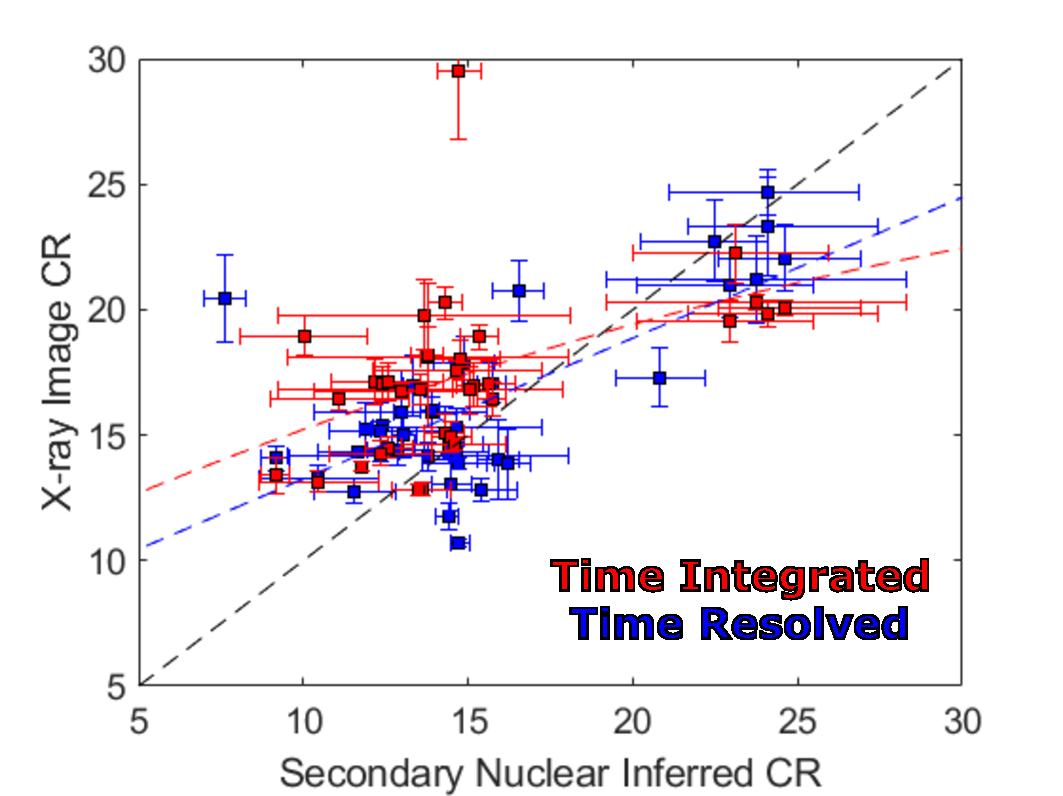
\includegraphics[scale=0.7]{Figures/xrayNuclearCR.pdf}
    \caption[Convergence Ratio Comparison]{Comparison of the convergence ratios inferred using secondary DT neutron yields and equatorial x-ray imaging techniques. Data shown in red corresponds to convergences inferred from time integrated images whereas data shown in blue corresponds to convergences inferred from time resolved x-ray images. In the case of time resolved images, the shape is inferred from the image with the greatest x-ray emission. Data is compiled from 58 different experiments on the NIF.}
    \label{fig:xraySecondaryComparison}
\end{figure}

As seen in Figure \ref{fig:xraySecondaryComparison}, the two methods do a decent job of tracing one another. However, there are clear discrepancies and a decent amount of scatter. X-ray images, on average, infer larger convergence ratios (infer a smaller hot-spot) for low convergence experiments (10-20). Interestingly, x-ray images infer smaller convergence ratios (infer a larger hot-spot) on average for large convergence experiments (20-30). \todo{This is likely because CH implosions have higher convergence. Maybe consider re plotting based on ablator if you have time.}

There are a handful of reasons why these discrepancies might be expected. First it's important to reiterate just how different the two methods are. The secondary neutron yield is really a measurement of a triton's average range in deuterium fuel while the x-ray image is a snapshot of the x-ray emitting region. Neither are a direct measurement of the fuel's peak convergence and both have (very different) sensitivities to other variables such as density profiles, temperature profiles, mix, and asymmetries. 



\begin{figure}
    \centering
    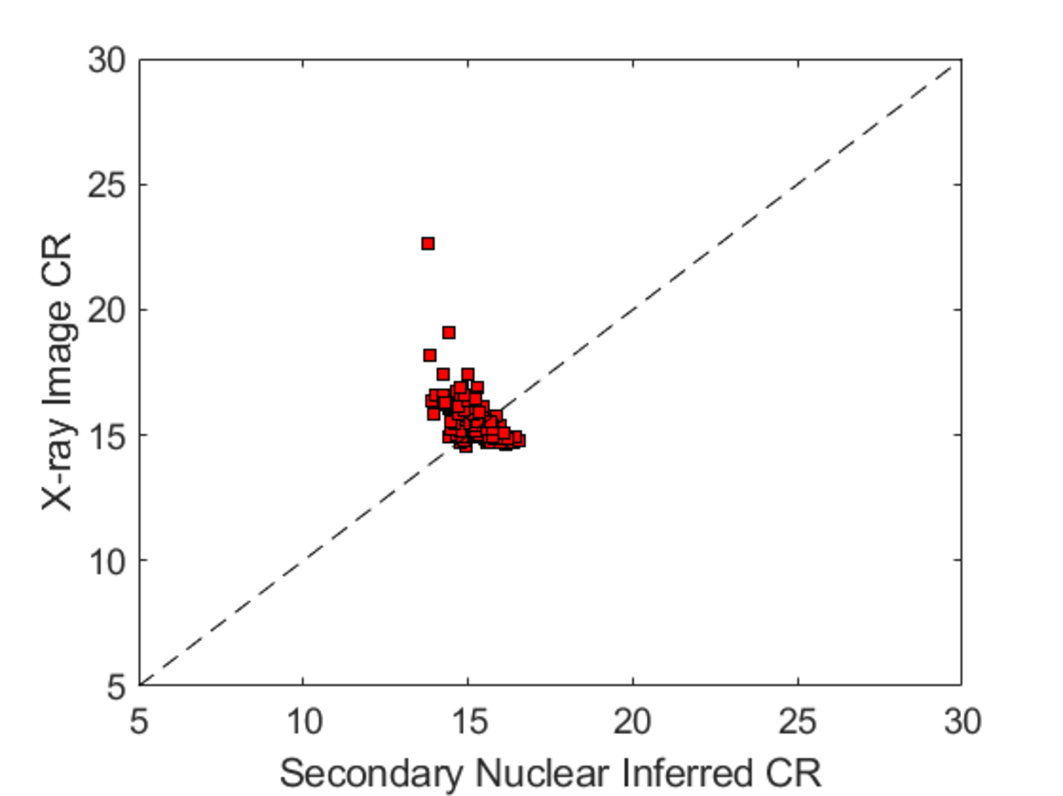
\includegraphics[scale=0.7]{Figures/noraXrayNucCR.pdf}
    \caption{Caption}
    \label{fig:}
\end{figure}

\subsection{Ryan Nora Simulations}



\begin{figure}
    \centering
    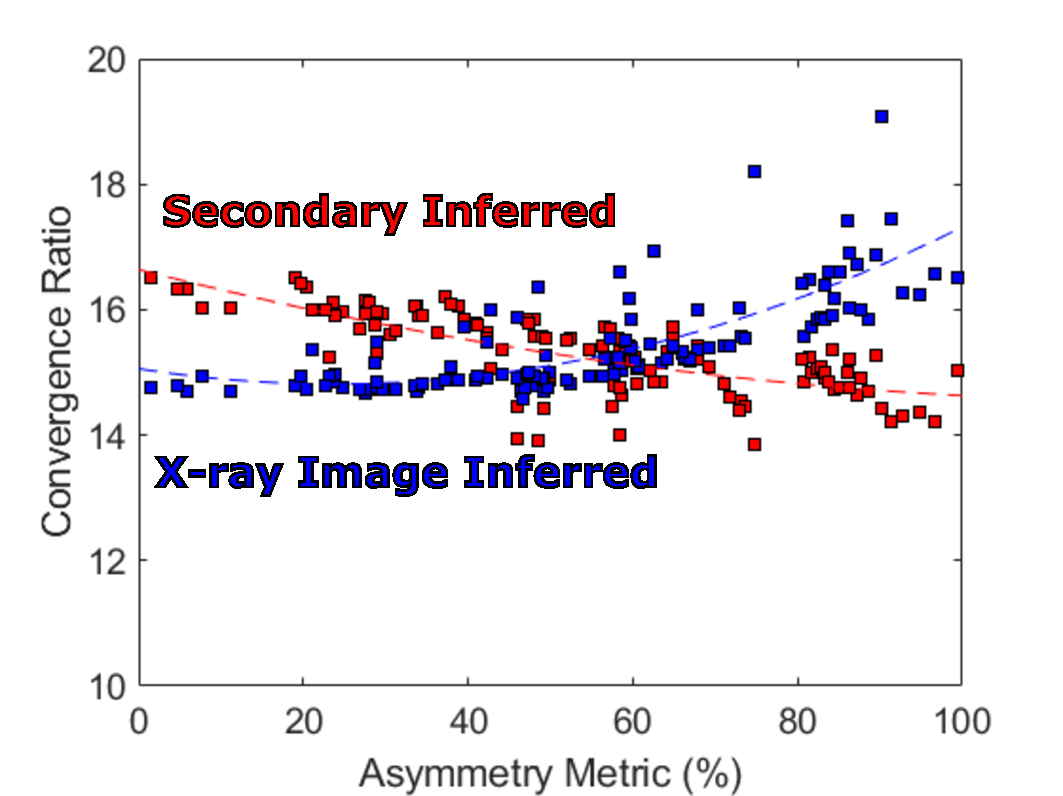
\includegraphics[scale=0.7]{Figures/noraXrayNucCRAsym.pdf}
    \caption{Caption}
    \label{fig:my_label}
\end{figure}
